%%=============================================================================
%% Methodologie
%%=============================================================================

\chapter{\IfLanguageName{dutch}{Methodologie}{Methodology}}
\label{ch:methodologie}

%% TODO: Hoe ben je te werk gegaan? Verdeel je onderzoek in grote fasen, en
%% licht in elke fase toe welke stappen je gevolgd hebt. Verantwoord waarom je
%% op deze manier te werk gegaan bent. Je moet kunnen aantonen dat je de best
%% mogelijke manier toegepast hebt om een antwoord te vinden op de
%% onderzoeksvraag.

\section{Proof of Concept}
\subsection{MS Dynamics 365FO}
Voor de Dynamics 365 implementatie werd een eigen module gebouwd. Een module kan volgens \textcite{Microsoft2019} beschouwd worden als een verzameling van elementen binnen MS Dynamics 365. 

Voor dit onderzoek werd gekozen voor module naam `chtbt'. In onderstaande figuur wordt een overzicht weergegeven van alle elementen waaruit de module bestaat. 

\subsubsection{Custom klassen}
Daar de voorgebouwde klassen in MSD365FO enorm veel data en logica bevatten, werd er voor gekozen om ook eigen klassen te maken. Dit werd gedaan adhv Table-extensions. De grootste motivatie hiervoor was dat die klassen (productieorder en bill of materials) ook serialiseerbaar moesten zijn om te kunnen versturen via web requests. Het is daarom niet verstandig om gigantische klassen te gaan serialiseren en versturen wanneer er slechts een fractie van de verstuurde gegevens nodig zijn. 

Ook was het nodig om deze klassen langs de client-kant (chatbot) te kunnen deserialiseren om CRUD-operaties mogelijk te maken. De deserialisatie werd geautomatiseerd, in die zin dat er gebruik werd gemaakt van Json2Csharp (zie 6.5.1). 

\subsubsection{Custom services}
Eens het datamodel gebouwd is, moeten de nodige methodes uiteraard beschikbaar zijn vanuit een third-party applicatie zoals de chatbot. Om dit te bewerkstelligen heeft men enkele opties (per \textcite{Microsoft2019a})

\begin{itemize}
    \item Custom Services
    \item OData Service
\end{itemize}

\textbf{OData Service:}\\ 
Deze manier van werken kan per \textcite{Microsoft2019b} gedefineerd worden als: 
een standaard protocol voor het creëren en consumeren van data. Het doel hiervan is om een standaard manier van werken aan te bieden die gebaseerd is op het REST protocol voor het creëren, lezen, updaten en deleten van data binnen D365FO. Ook maakt de service gebruik van JSON voor het versturen van informatie. 

In de werkelijkheid komt het erop neer dat men vanuit third party apps queries kan uitvoeren en versturen naar D365FO. Een voorbeeld hiervan kan geraadpleegd worden op onderstaande afbeeldingen.

\begin{figure}[H]
    \centering
    \includegraphics[width=1\textwidth]{img/ODataExample}
    \caption{data creatie voor een create operatie adhv OData binnen D365FO \cite{Lanssens2018}}
    
\end{figure}

\begin{figure}[H]
    \centering
    \includegraphics[width=1\textwidth]{img/ODataExample2}
\caption{webrequest creatie en versturing voor een create operatie adhv OData binnen D365FO \cite{Lanssens2018}}
\end{figure}

\textbf{Custom Services}\\
Voor dit onderzoek werd er voor gekozen om niet gebruik te maken van Odata Servies, maar van Custom Services. Dit wil zeggen dat men langs D365FO's kant zelf services gaat definiëren, en deze beschikbaar gaat stellen via hun eigen endpoint. Deze manier van werken is iets overzichtelijker wanneer er van de buitenwereld gebruikt wordt gemaakt van custom methodes binnen D365FO die een of meerde parameters verwachten. In D365FO hoeft men enkel te definiëren welke parameters binnenkomen, en deze te verwerken, Terwijl in de third party app (bot) slechts de juiste endpoints moeten worden aangesproken samen met de nodige parameters. 

Een handleiding in detail van hoe dit werd gerealiseerd kan worden teruggevonden in de bijlagen (bijlage D).


\subsection{Authenticatie Applicatie}
Zoals gezegd werd er doelbewust gekozen om het authenticatiegedeelte te encapsuleren in een aparte applicatie. Dit om gevoelige informatie, zoals connectiesleutels etc., te kunnen verbergen van de buitenwereld. 

Maar verder is deze manier van werken interessant, omdat meerdere bots deze zouden kunnen gebruiken, maar ook andere third-party apps (zoals bv. een mobiele app) zouden in principe dankzij deze tussenapplicatie kunnen connecteren met D365FO. 

\subsection{MS Bot Framework implementatie}
\subsubsection{Bot zelf}
Dankzij Azure is het aanmaken van een nieuwe bot relatief eenvoudig. Zo zal de portaal automatisch alle benodigde resources aanmaken en configureren voor de nieuw aangemaakte bot.\\

Voor dit onderzoek werd gekozen voor een Web App Bot (template: Basic Bot) van SDK 4. Dit is de meest recente (2019), en implementeert LUIS al gedeeltelijk. Dit is een ideaal vertrekpunt voor een nieuwe chatbot die natuurlijke taal verwerkt en beantwoordt met gepaste verlopen specifiek per casus. 

Een handleiding in detail van hoe dit werd gerealiseerd kan worden teruggevonden in de bijlagen (bijlage B).

Dankzij het waterval-principe 

\subsubsection{NLP}
Uiteraard is één van de kerncomponenten van een chatbot natural language processing (NLP). In het Microsoft Bot Framework wordt LUIS gebruikt als engine om natuurlijke taal om te zetten naar bruikbare commando's die elk hun eigen invulling vereisen.\\ 

\rightline{\textbf{Werking}}
Voor de werking rust LUIS op 2 kernbegrippen. Intenties enerzijds, en Entiteiten anderzijds. Intenties worden gebruikt om aan te duiden wat de gebruiker wilt doen. Zo zal een chatbot anders reageren als een gebruiker wilt weten hoelaat het is, dan indien hij het weer voor die dag zou opvragen.\\
\rightline{Intenties:}\\
Deze component wordt gebruikt om een bot op te delen in verschillende functionaliteiten. Elke intentie zal zijn eigen vervolg geven aan het bericht van de gebruiker. Zo zal het verloop bij de intentie `GeefWeer' anders reageren dan bij de intentie 'GeefProductieOrders'. 

Wanneer men een LUIS app maakt kan men intenties opgeven, en hier voorbeeldzinnen aan toevoegen. De service zal dan automatisch op basis van de voorbeeldzinnen het model trainen (Machine Learning). Hierna kunnen zinnen naar LUIS verstuurd worden, en LUIS zal dan voor elke zin een score gaan berekenen per intentie. Met andere woorden: hoe groot is de kans dat de gebruiker met zin 'x' intentie 'y' wil bereiken. De intentie die hier het hoogst op scoort zal gekozen worden, en vervolgens teruggestuurd worden. 
Op onderstaande figuur wordt een illustratief maar niet limitatief voorbeeld weergegeven. 

\begin{figure}[H]
    \centering
    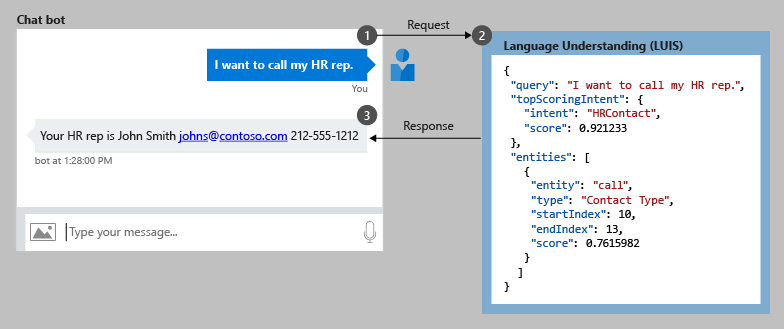
\includegraphics[width=1\textwidth]{img/LuisIntents}
\caption{voorbeeld van een LUIS respons \cite{Microsoft2019c}}
\end{figure}

\rightline{Entiteiten:}
Wanneer men NLP wil bereiken op een efficiënte manier, zal men ook enige notie moeten hebben van entiteiten. Onder deze term wordt alle bijkomende informatie, die van belang is, verzameld. Zo is het bijvoorbeeld niet enkel nodig om te weten dat een gebruiker het weer wil zien, maar ook van welke dag. Net zoals dat het niet enkel handig is om te weten dat de gebruiker een productie order wil bekijken, maar ook het productie order nummer in kwestie zal vereist zijn.
Ook hier treedt een vorm van artificiële intelligentie op. Zo zal LUIS immers automatisch herkennen of er entiteiten aanwezig zijn in een zin, en deze terugsturen met zijn antwoord. Uiteraard is dit niet vanzelfsprekend, en verwacht LUIS ook hier dat je de service eerst traint. Dit doet men door de nodige entiteiten te definiëren. Hiervoor heeft de developer verschillende keuzes. Zo is het mogelijk om een entiteit te definiëren aan de hand van patronen, reguliere expressies, composities, etc. \\
Op onderstaande figuur wordt weergegeven hoe een compositie eruit ziet. We zien dat er 3 entiteiten (number, PassengerClass en Travelclass) gedefinieerd zijn. Dankzij voorbeelden van elke entiteit en training is LUIS in staat de entiteiten te herkennen, en automatisch toe te voegen aan de compositie.

\begin{figure}[h]
    \centering
    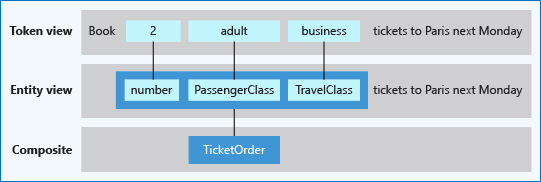
\includegraphics[width=0.8\textwidth]{img/LuisEntities}
    \caption{voorbeeld van LUIS entiteiten \cite{Microsoftd}}
    \end{figure}

Een handleiding in detail van hoe dit werd gerealiseerd voor deze poc kan worden teruggevonden in de bijlagen (bijlage C).

----------------------------------------------------------
\section{Onderzoek}
Aangezien het meten van onderzoeksvraag B nogal lastig is (Er zijn weinig meetbare parameters om dit te kunnen bevestigen/ontkrachten). Daarom werd er in dit onderzoek voor gekozen om een bevraging te doen naar de meningen van gebruikers. Voor het afnemen van de enquête werd er een demo en uitleg gegeven bij het doorlopen van 1 funtionaliteit (productieorder opzoeken \& starten). Vervolgens werd een bevraging gedaan naar beide systemen op vlak van: 

\begin{itemize}
    \item gebruiksvriendelijkheid
    \item eenduidigheid
    \item tijdverlies
\end{itemize}

\subsection{Vragenlijst}
onder deze noemers wordt het volgende verstaan:

\textbf{eenduidigheid}\\
Alles is duidelijk omschreven, er heerst geen onduidelijkheid over wat welke knop/stap teweeg zal brengen.\\

\textbf{gebruiksvriendelijkheid}\\
Het systeem voelt intuïtief en robuust aan. De gebruiker heeft steeds het gevoel dat hij de controle heeft.\\

\textbf{tijdverlies}\\
De gebruiker moet lang wachten tussen clicks in, het duurt trager dan dat het zou mogen duren.

Zo werd er gevraagd om steeds een score te geven van 1-5. Elke gebruiker heeft dus 6 scores opgegeven. Tenslotte werd er ook bij elk systeem (D365 vs chatbot) gevraagd of er opmerkingen/feedback waren.
in onderstaande figuur vind men een overzicht terug van de gebruikers, en hun scores.  


\subsection{Resultaten}
Op figuur 7.1 kan een overzicht worden teruggevonden van de onderzoeksresultaten. Voor meer info over de enquête kunnen de bijlagen geraadpleegd worden (bijlage f). 
\begin{table}[]
    \begin{tabular}{llll}
        \cline{1-2}
        \multicolumn{1}{|l|}{Gebruikers}                                   & \multicolumn{1}{l|}{aantal} &                              &                                                \\ \cline{1-2}
        \multicolumn{1}{|l|}{Met voorkennis D365FO (medewerkers delaware)} & \multicolumn{1}{l|}{14}     &                              &                                                \\ \cline{1-2}
        \multicolumn{1}{|l|}{Zonder voorkennis D365FO}                     & \multicolumn{1}{l|}{6}      &                              &                                                \\ \cline{1-2}
        \multicolumn{1}{|l|}{Totaal}                                       & \multicolumn{1}{l|}{20}     &                              &                                                \\ \cline{1-2}
        &                             &                              &                                                \\ \hline
        \multicolumn{1}{|l|}{\textbf{gemiddelden}}                         & \multicolumn{1}{l|}{D365FO} & \multicolumn{1}{l|}{Chatbot} & \multicolumn{1}{l|}{Verschil (D365FO-Chatbot)} \\ \hline
        \multicolumn{1}{|l|}{Gebruiksvriendelijkheid}                      & \multicolumn{1}{l|}{3.36}   & \multicolumn{1}{l|}{4.27}    & \multicolumn{1}{l|}{-0.93}                     \\ \hline
        \multicolumn{1}{|l|}{Eenduidigheid}                                & \multicolumn{1}{l|}{3.43}   & \multicolumn{1}{l|}{3.86}    & \multicolumn{1}{l|}{-0.43}                     \\ \hline
        \multicolumn{1}{|l|}{Tijdverlies}                                  & \multicolumn{1}{l|}{3.30}   & \multicolumn{1}{l|}{3.00}    & \multicolumn{1}{l|}{0.29}                      \\ \hline
    \end{tabular}
\caption{\label{tab:Overzicht bevraging Dynamics 365FO vs Chatbot}Overzicht bevraging Dynamics 365FO vs Chatbot}
\end{table}

\subsection{conclusie}
Men merkt al snel op dat de chatbot voor gebruiksvriendelijkheid bijna 1 punt (0.93) beter scoort dan Dynamics 365FO. Ook voor Eenduidigheid en tijdverlies presteert de chatbot respectievelijk 0,43 en 0.29 punten beter dan Dynamics. Alhoewel dit vrij aanzienlijk is op 20 bevragingen, moet men rekening houden met het aantal bevragingen. Verder blijft het een kwestie van meningen, en dus geen exacte wetenschap. 

